\documentclass[aspectratio=169]{beamer}

\mode<presentation> {
    \usetheme{Madrid}
    \usecolortheme{rose}
}

\usepackage{graphicx}
\usepackage{booktabs}
\usepackage{subfigure}
\usepackage[bookmarks=true]{hyperref}
\usefonttheme{serif}

\title[Scaling Laws]{
    Exploring Scaling Laws in LLM Pretraining
}

\author{Zibo Ren, Runlin Chen}
\institute[PKU]
{
    Peking University \\
    \medskip
    \texttt{\{2200010626,2200010848\}@stu.pku.edu.cn}
}
\date{\today}

\begin{document}

\begin{frame}
    \titlepage
\end{frame}

\begin{frame}
    \frametitle{Overview}
    \tableofcontents
\end{frame}

\section{Scaling Laws}\label{sec:scalinglaws}

\subsection{Chinchilla Scaling Law}\label{subsec:chinchilla}
\begin{frame}
    \frametitle{Chinchilla Scaling Law}
    \begin{block}{Chinchilla Scaling Law}
        \begin{equation}
            \label{eq:chinchilla}
            \begin{aligned}
                L(D, N) &= L_0 + A\cdot D^{-\alpha} + B\cdot N^{-\beta} \\
            \end{aligned}
        \end{equation}
    \end{block}
    \begin{itemize}
        \item $L(D, N)$ is the final validation loss.
        \item $D$ is the amount of data.
        \item $N$ is the number of parameters.
        \item $L_0$, $A$, $B$, $\alpha$ and $\beta$ are undetermined
            positive constants.
    \end{itemize}

    It only illustrates the loss at the end of training, but not the
    loss during training.
\end{frame}

\subsection{Scaling Law with LR Annealing (LRA)}\label{subsec:LRA}

\begin{frame}
    \frametitle{Scaling Law with LR Annealing}
    \begin{block}{Scaling Low Formula}
        \begin{equation}
            \label{eq:scaling_low}
            \begin{aligned}
                L(s) &= L_0 + A\cdot S_1^{-\alpha} - C\cdot S_2 \\
                S_1 &= \sum_{i=1}^{s} \eta_i \\
                S_2 &= \sum_{i=1}^{s} \sum_{k=1}^{i} (\eta_{k-1} -
                \eta_k)\cdot\lambda^{i-k}
            \end{aligned}
        \end{equation}
    \end{block}

    \begin{enumerate}
        \item $L(s)$: the loss at step $s$.
        \item $\eta_i$: the learning rate at step $i$.
        \item $\lambda$: a hyper-parameter to notate the decay factor
            in LR annealing momentum.
    \end{enumerate}
\end{frame}

\begin{frame}
    \frametitle{Defect of Scaling Law with LR Annealing}
    \begin{enumerate}
        \item If the we add some iterations with learning rate 0 to
            the end of the training, according to
            (\ref{eq:scaling_low}), the loss will still decrease dual
            to $S_1$ is not change and $S_2$ is increasing.
        \item The form of $S_2$ is based on observation, but it is lack of
            theoretical support.
    \end{enumerate}
\end{frame}

\subsection{Multi-Power Law}\label{subsec:MPL}

\begin{frame}
    \frametitle{Multi-Power Law}
    \begin{block}{Multi-Power Law}
        \begin{equation}
            \label{eq:multi_power_law}
            \begin{aligned}
                &L(t) = L_0 + A\cdot (S_1(t) + S_W)^{-\alpha} - LD(t)\\
                &\text{where} \\
                & LD(t) = B\sum_{k=1}^{t}(\eta_{k-1}-\eta_k)\cdot
                G(\eta_k^{-\gamma}S_k(t)), \\
                &S_k(t) = \sum_{i=k}^{t} \eta_i, \\
                &G(x) = 1-(Cx+1)^{-\beta}
            \end{aligned}
        \end{equation}
    \end{block}

    \begin{enumerate}
        \item $A\cdot (S_1(t) + S_W)^{-\alpha}$ is an extension of
            Chinchilla scaling law.
        \item $LD(t)$ is a correction term to account for the
            learning rate decay.
        \item Actually $G(x)$ can be any increasing function that
            maps $[0, \inf]$ to $[0, 1]$.
    \end{enumerate}
\end{frame}

\section{Experiments}\label{sec:experiments}

\begin{frame}
    \frametitle{Experiments Setup}
    \begin{enumerate}
        \item We use the loss curves of a 100M GPT model trained on
            20B tokens of data.
        \item We use 3 types of learning rate schedules: "8-1-1",
            warmup-stable-decay(WSD) and cosine.
        \item The total train step is 33907, we use the first 10000
            of one learning rate schedule to fit the parameters of
            the model and test the model on the full loss curve of
            the three learning rate schedules.
    \end{enumerate}
\end{frame}

\begin{frame}
    \frametitle{Experiments Results of LRA}
    We use cosine learning rate schedule to fit the parameters
    \begin{figure}
        \centering
        \subfigure[cosine learning rate]{
            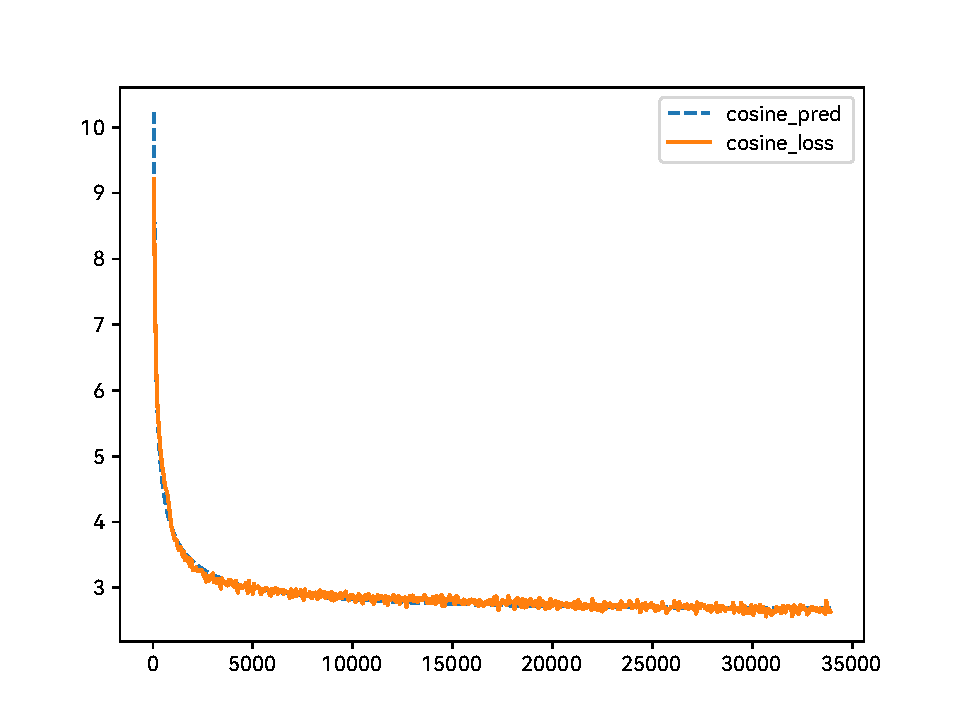
\includegraphics[width=0.3\textwidth]{fig/lra/cosine_fit.pdf}
        }
        \subfigure[8-1-1 learning rate]{
            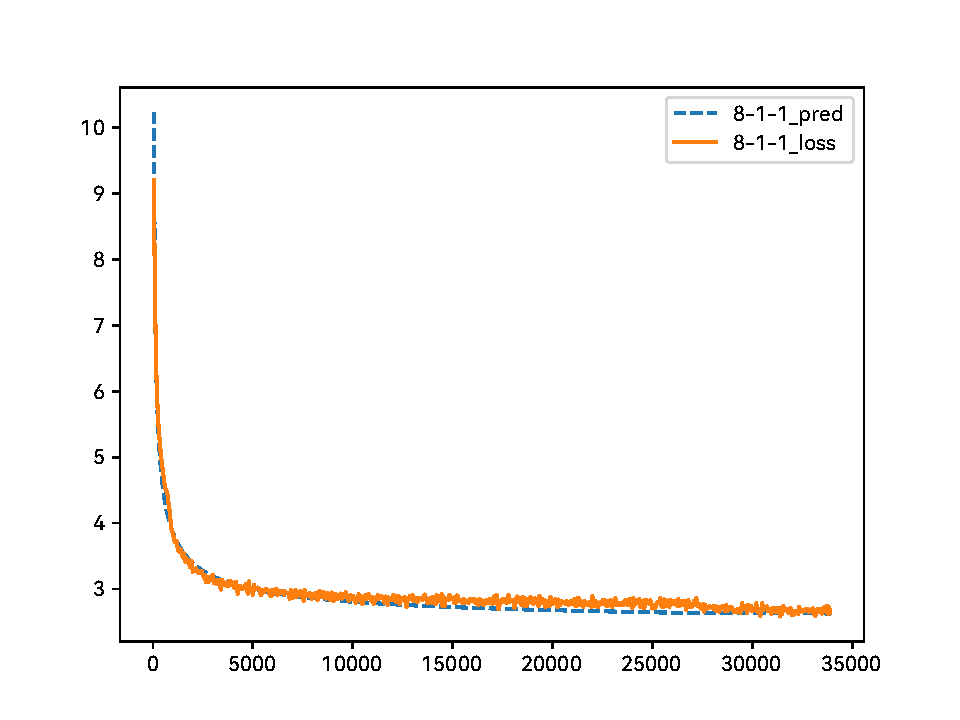
\includegraphics[width=0.3\textwidth]{fig/lra/8-1-1_fit.pdf}
        }
        \subfigure[WSD learning rate]{
            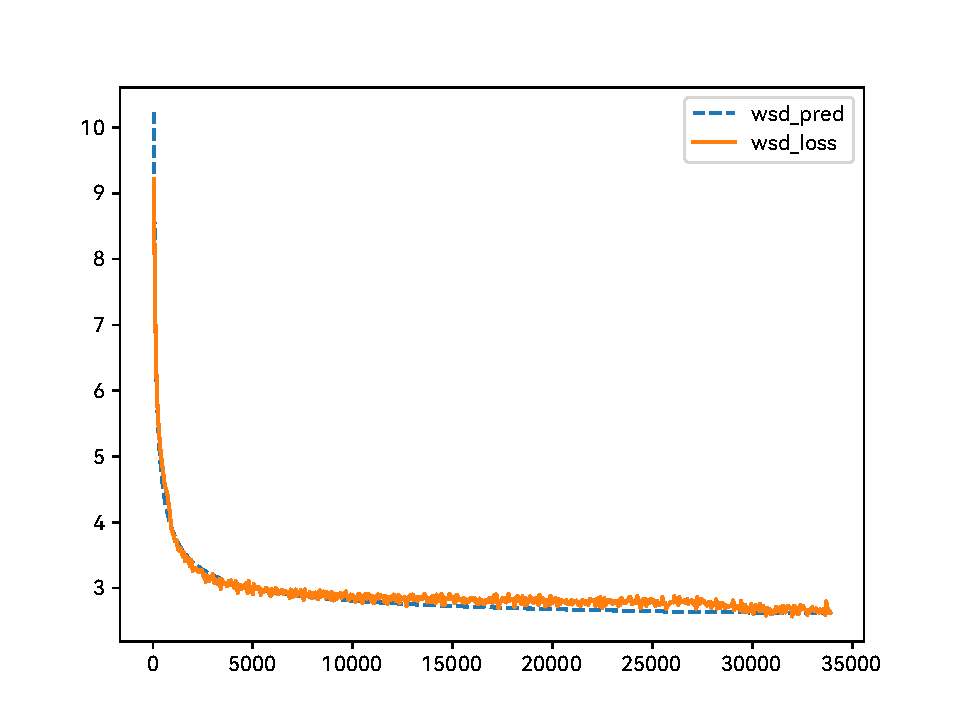
\includegraphics[width=0.3\textwidth]{fig/lra/wsd_fit.pdf}
        }
    \end{figure}
\end{frame}

\begin{frame}
    \frametitle{Experiments Results of MPL}
    We use cosine learning rate schedule to fit the parameters
    \begin{figure}
        \centering
        \subfigure[cosine learning rate]{
            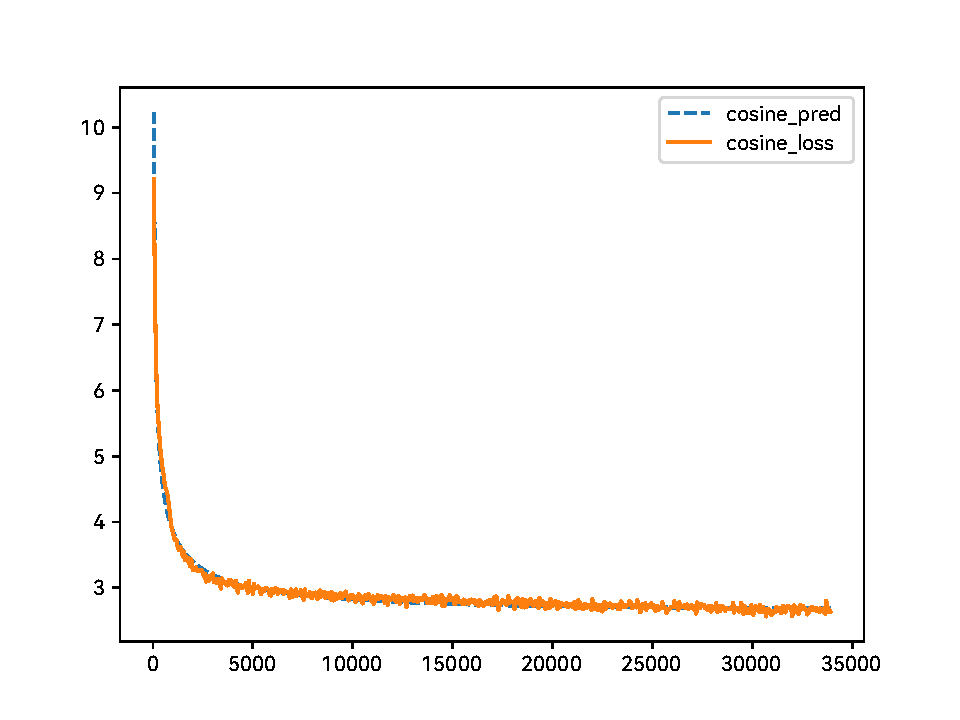
\includegraphics[width=0.3\textwidth]{fig/mpl/cosine_fit.pdf}
        }
        \subfigure[8-1-1 learning rate]{
            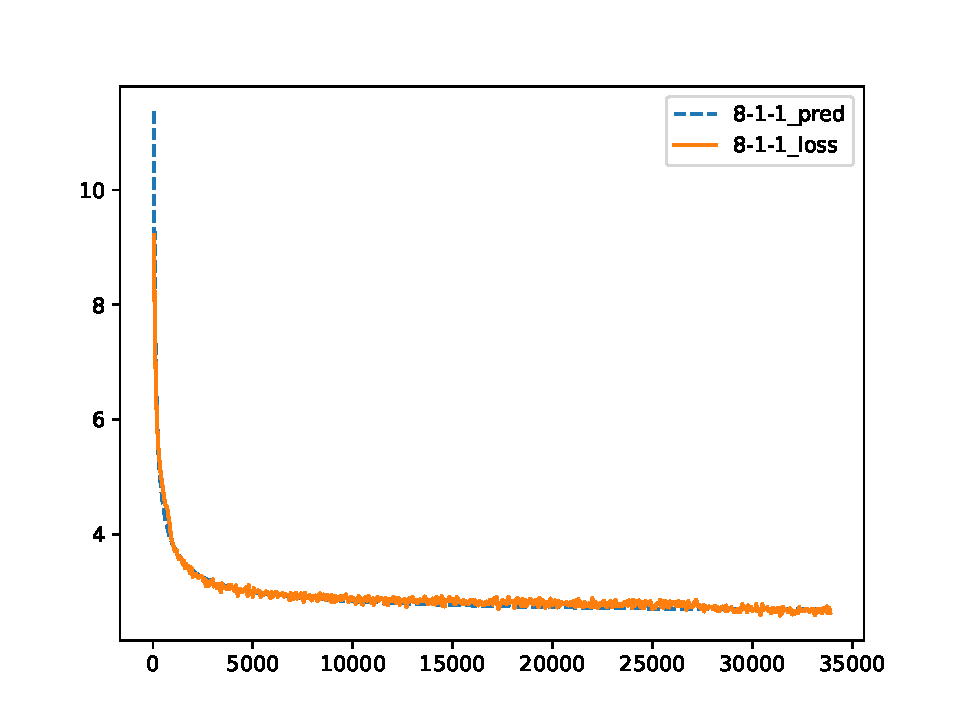
\includegraphics[width=0.3\textwidth]{fig/mpl/8-1-1_fit.pdf}
        }
        \subfigure[WSD learning rate]{
            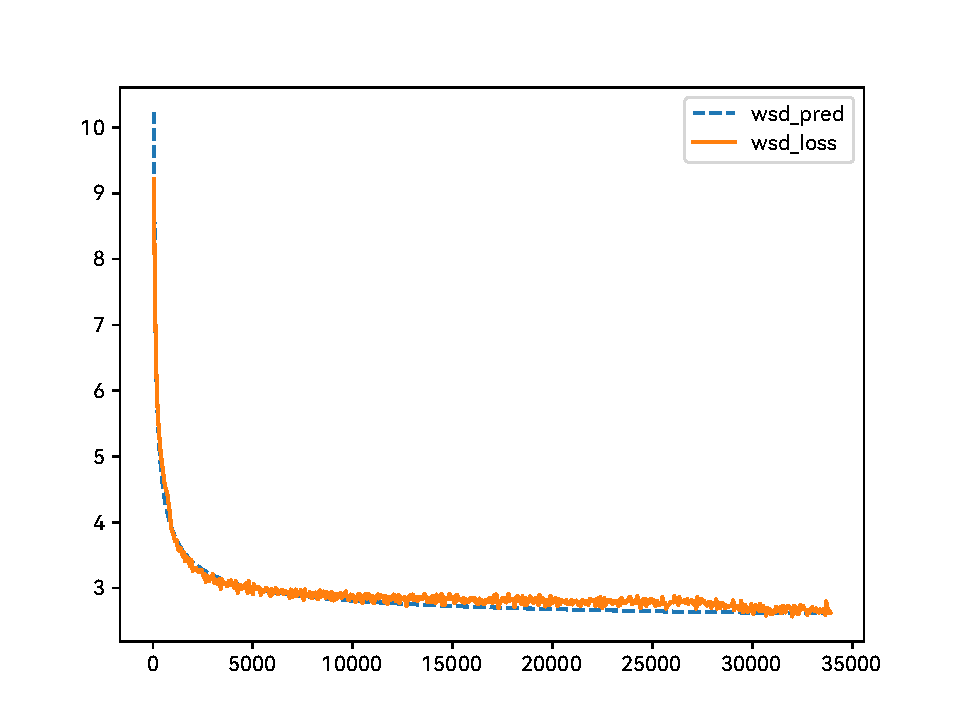
\includegraphics[width=0.3\textwidth]{fig/mpl/wsd_fit.pdf}
        }
    \end{figure}
\end{frame}

\section{Flaws in Scaling Laws}\label{sec:flaws}

\end{document}